\section{MicroSims: Definition and Characteristics}
\label{sec:definition}

\subsection{Formal Definition}

We define an \textit{Educational MicroSim} as a lightweight, standalone interactive simulation that executes within standard web browsers and is specifically designed for pedagogical applications. Educational MicroSims are characterized by their focused scope, browser-native implementation, and compatibility with generative AI systems. They occupy a unique position at the intersection of simplicity, accessibility, and AI-generation capability, providing an optimal balance of interactivity and pedagogical effectiveness.

\begin{figure}[htbp]
\centering
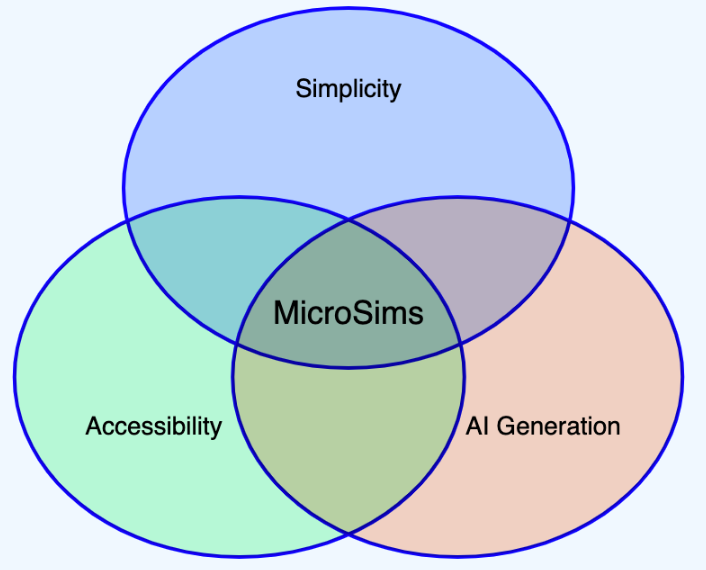
\includegraphics[width=0.6\textwidth]{figures/microsim-uniqueness.png}
\caption{MicroSims occupy a unique position at the intersection of three critical characteristics: Simplicity (lightweight, focused scope), Accessibility (browser-based, universal embedding), and AI Generation (standardized patterns, prompt-compatible). This convergence of attributes distinguishes MicroSims from other educational technology approaches and enables their scalable deployment across diverse learning contexts.}
\label{fig:uniqueness}
\end{figure}

\subsection{Core Characteristics}

\textbf{Focused Scope}: MicroSims deliberately constrain their focus to specific learning objectives rather than attempting comprehensive coverage of broad subject domains.

\textbf{Browser-Native}: All MicroSims run entirely in web browsers using HTML5, CSS, and JavaScript, requiring no installation or specialized software.

\textbf{Generative AI Compatible}: MicroSims follow standardized design patterns that enable large language models to generate, modify, and extend them based on natural language descriptions.

\textbf{Universal Embedding}: Through iframe architecture, MicroSims can be embedded in any digital environment that supports web content.

\textbf{Transparent Implementation}: MicroSim code is intentionally readable and well-documented, enabling educators and students to examine, understand, and modify the underlying logic.

\subsection{Technical Architecture}

MicroSims are implemented as self-contained web applications, typically using JavaScript frameworks such as p5.js, that require no external dependencies or server-side infrastructure. They follow a standardized width-responsive design pattern with distinct regions for visualization (drawing area) and user controls (interaction area). The layout of MicroSims can be expressed in rules files that are used by generative AI systems to ensure consistent implementation patterns across different simulations.

\begin{figure}[htbp]
\centering
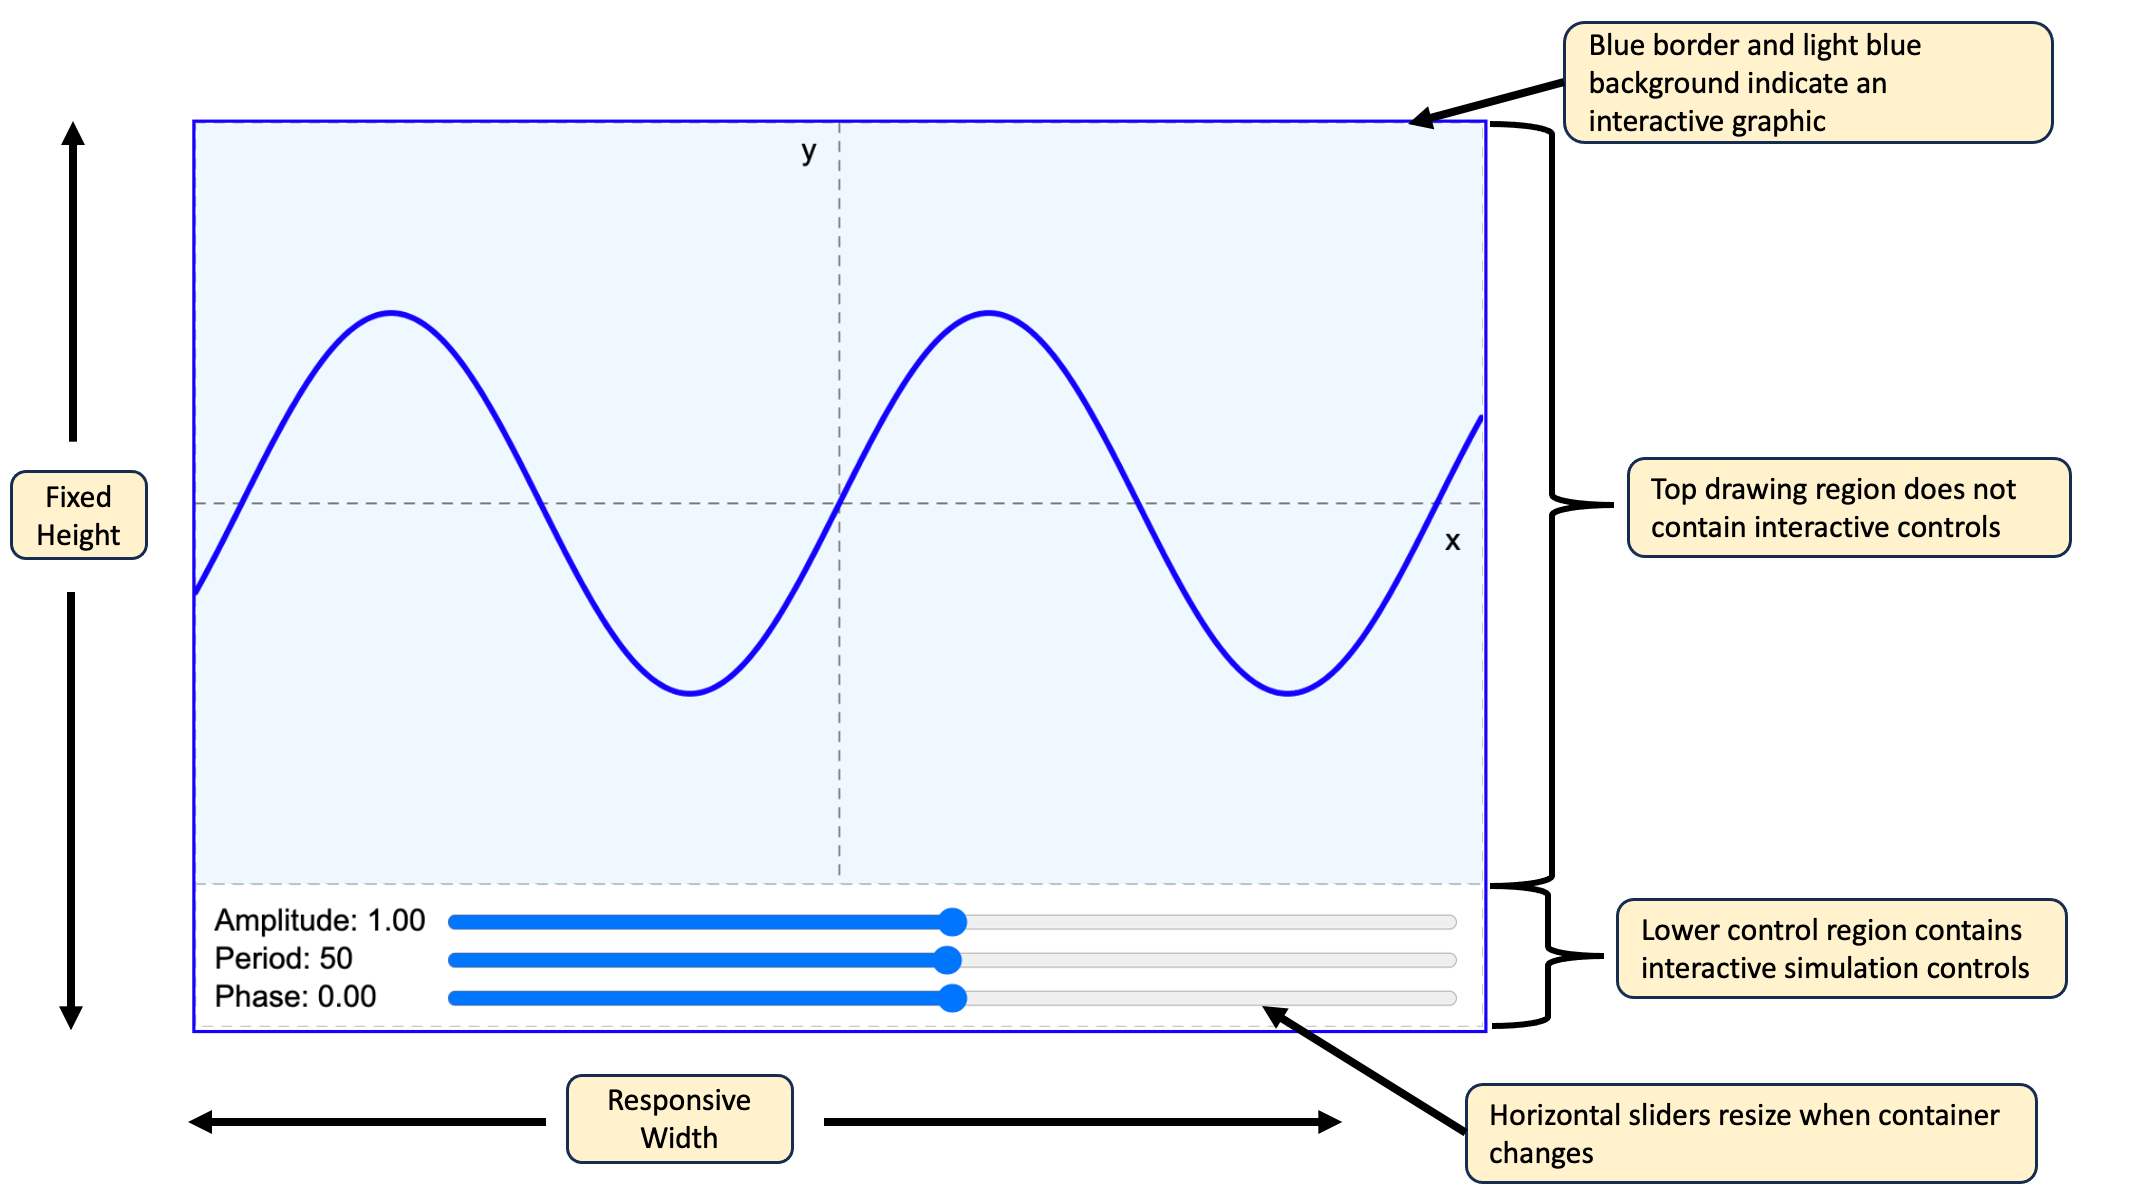
\includegraphics[width=0.6\textwidth]{figures/microsim-layout.png}
\caption{MicroSims use a standardized layout pattern with distinct areas for visualization and user controls. This consistent structure facilitates generative AI creation and modification of MicroSims while ensuring usability across diverse educational contexts.  This layout consistency also allows interactivity to be logged in a standardized way for integration with intelligent textbooks and learning analytics systems.}
\label{fig:layout}
\end{figure}



Being browser-based and dependency-free, MicroSims can be easily distributed, embedded in various learning management systems, and accessed across different devices and platforms without installation requirements. The goal is to allow a MicroSim to be placed on any web page using a single HTML \texttt{iframe} element.

\subsection{Educational Purpose and Learning Objectives}

Each MicroSim targets specific learning objectives within a curriculum, enabling students to manipulate parameters and observe resulting changes in real-time. They support experiential learning by allowing learners to explore cause-and-effect relationships through direct interaction with underlying models or algorithms.

The simulations are engineered for modification and extension by non-technical users including educators, students, and content creators. They employ consistent user interface conventions and well-documented code structures to facilitate customization without requiring advanced programming expertise.

MicroSims generate structured event streams capturing user interactions, parameter adjustments, and exploration patterns. These data streams can be analyzed to assess learning progress and provide feedback to adaptive educational systems, including intelligent textbooks that employ reinforcement learning to optimize the learning experience.

\subsection{Scope Boundaries: What MicroSims Are Not}

To clarify the scope and boundaries of Educational MicroSims, it is important to establish what they explicitly are not:

\textbf{Not Simple Animations}: MicroSims are not simple animations of educational concepts. Although generative AI can create beautiful animations, without some student action required for participation, we cannot use feedback and reinforcement learning in intelligent textbooks. Simulations must at a minimum contain interactive controls such as ``Start'' and ``Pause'' buttons. Monitoring user interactions with these controls is critical for the development of intelligent textbooks.

\textbf{Not Technology-Dependent}: MicroSims are not bound to any specific JavaScript library or framework. While our implementation examples utilize p5.js for its pedagogical clarity and ease of use, the MicroSim concept is library-agnostic and can be implemented using vanilla JavaScript, D3.js, Three.js, or any other web-based rendering technology that meets the functional requirements.

\textbf{Not Legacy Standards Compliant}: MicroSims do not adhere to traditional e-learning standards such as SCORM (Sharable Content Object Reference Model) or AICC (Aviation Industry Computer-Based Training Committee). These legacy standards impose architectural constraints and complexity that are incompatible with the lightweight, generative nature of MicroSims. However, because MicroSims all have interactive controls, they can be designed to easily work with xAPI standards, and generative AI can be used to automatically add xAPI calls to the controls area.

\textbf{Not Comprehensive Simulation Environments}: MicroSims are not intended to replace complex, full-featured simulation platforms or virtual laboratories. They are purposefully constrained in scope to address specific, well-defined learning objectives rather than attempting to model entire systems or domains.

\textbf{Not Platform-Specific Applications}: Unlike native mobile applications or desktop software, MicroSims are not tied to specific operating systems or device types. They maintain platform independence through adherence to web standards and responsive design principles.

\textbf{Not Server-Dependent Systems}: MicroSims do not require server-side processing, databases, or cloud infrastructure for their core functionality. While they may optionally integrate with learning analytics platforms, their primary operation remains entirely client-side.

\subsection{Metadata Strategy}

MicroSims leverage established metadata standards where appropriate to enable proper cataloging, discovery, and interoperability within educational repositories and learning management systems. They incorporate Dublin Core metadata elements for resource description, providing standardized fields for title, creator, subject, description, date, type, format, language, and rights information.

This metadata strategy ensures that MicroSims can be systematically organized, searched, and integrated into existing educational technology infrastructures while maintaining their lightweight, generative characteristics. The metadata framework supports both human curation and automated discovery processes, facilitating the scalable deployment of MicroSim collections across diverse educational contexts.

This definition establishes MicroSims as a distinct category of educational technology that bridges the gap between static educational content and complex simulation environments, providing an optimal balance of interactivity, accessibility, and pedagogical effectiveness.
